\subsubsection{UC1 - Visualizzazione guida introduttiva}
	\begin{figure}[h]
		\centering
		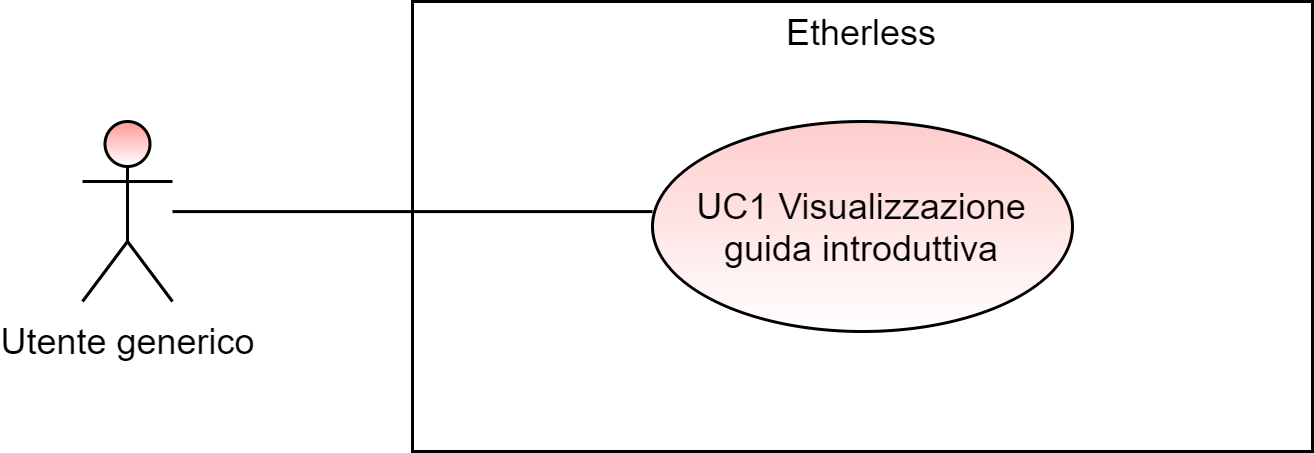
\includegraphics[scale=\ucs]{./res/img/UC1G.png}
		\caption {UC1 - Visualizzazione guida introduttiva}
	\end{figure}
	\begin{itemize}
		\item \textbf{Attori primari:} \ug{};
		\item \textbf{Descrizione:} dopo aver eseguito il comando \init{} il sistema mostra una guida contenente una breve spiegazione riguardante i comandi di \login{} e \signup{}. Tale guida ha lo scopo di aiutare l'utente a procedere nell'utilizzo dell'applicativo; 
		\item \textbf{Scenario principale:} 
		\begin{itemize}
			\item l’utente inserisce il comando \init{};
			\item viene visualizzata la guida introduttiva.
		\end{itemize}
		\item \textbf{Precondizione:} l'applicativo viene avviato correttamente e il sistema è raggiungibile;
		\item \textbf{Postcondizione:} vengono fornite all'utente tutte le informazioni necessarie per procedere con l'utilizzo dell'applicativo. 
	\end{itemize}